\section{Case Studies}
\label{sec:evaluation}
This section describes how we evaluated our model through two case studies of existing software development security data.

We presented the data elements to be collected for our full model in Section ~\ref{sec:model_measurement}, and the data collection guide for the measurement model gives instructions on how to collect the data for a software development project~\cite{morrison2016spefsite}.  SEM is a large-sample technique, with median sample size in the literature of 200 observations~\cite{kline2015principles}. The need for large quantities of software development security data leads us to examine existing software development security datasets. Further, confirmation of our hypothesized structural and measurement relationships in data we did not generate would strengthen the case for the theorized relationships.
We have identified two candidate data sets, of increasing detail and decreasing observation count: 
\begin{itemize}
\item The NVD contains vulnerability records for a wide variety of software, over a long timespan.
\item The CII project census contains high-level project data for over 400 Debian~\footnote{https://www.debian.org/} packages.
\end{itemize}

For each dataset, the project is our unit of analysis. In the case of the NVD, which reports vulnerabilities, we collect all vulnerabilities for a given project and summarize them. Each CII record represents a single project. We assume the data points collected for each project in both datasets are independent of other projects.  We give further details for each of these datasets in their case study sections, below. We used the R~\footnote{https://www.r-project.org} lavaan package to conduct our SEM analysis, as well as the ggplot2, semPlot and psych R packages. We now introduce the lavaan syntax, and explain the semantics of each syntax element.

\begin{itemize}
\item Regression relationships between latent variables are specified using the $\sim$  operator (see Table \ref{tab:model_lavaan_syntax}), for example $Outcomes \sim SoftwareRisk + AssetImpact$ (SoftwareRisk is also modeled as affecting Outcomes) ("Outcomes are dependent on Software Risk and Asset Impact"). Establishing a parameter estimate for this relationship allows us to test hypotheses about the latent variable relationships, for example the hypothesis that \textbf{H1} Asset Impact is associated with negative Security Outcomes.
 \item Covariance relationships are specified using the $\sim\sim$ operator.
\item Latent variable-measurement variable relationships are specified as follows: $LatentVariable =\sim MeasuredVariable1 + ...$. 
\item Dashed lines indicate estimates established by the modeler, or by the software. We have two examples of modeled fixed parameters in our structural model: We specify the absence of a direct relationship between Asset Impact and Software Risk (syntax: $SoftwareRisk \sim\sim 0*AssetImpact$), as we expect the constructs to be independent of each other. We specify the absence of a direct relationship between Adherence and Outcomes, as we expect Adherence to affect Outcomes through being moderated by overall Software Risk. The remaining dashed lines are estimates fixed by the software, where it has estimated starting values in the course of solving the system of equations expressed by the model.
\end{itemize}

We now present the complete set of structural model contstructs and relationships, first in English, then in the lavaan model syntax: 
 
 "Software Risk is measured by Software Context Factors"
 \begin{equation} \label{eq:0}
 \begin{split}
 SoftwareRisk &=\sim SoftwareContextFactors 
 \end{split}
 \end{equation}

"Asset Impact is measured by Asset Context Factors"       
 \begin{equation} \label{eq:1}
 $AssetImpact =\sim AssetContextFactors$
 \end{equation}
 
 \begin{equation} \label{eq:1}
 \begin{split}
 AssetImpact &=\sim AssetContextFactors 
        - "Asset Impact is measured by Asset Context Factors"\\
 Outcomes &=\sim OutcomesContextFactors "Outcomes are measured by Outcome Context Factors\\ 
 Adherence &=\sim AdherenceContextFactors "Adherence is measured by Adherence Context Factors"\\
 Outcomes &\sim SoftwareRisk + AssetImpact "Outcomes are dependent on Software Risk and Asset Impact"\\
 SoftwareRisk &\sim Adherence "Software Risk is dependent on Adherence"\\
 AssetImpact &\sim\sim  Adherence "Asset Impact is correlated with Adherence"\\
 SoftwareRisk &\sim\sim 0*AssetImpact "Software Risk and Asset Impact are not directly correlated."\\
 Adherence &\sim\sim 0*Outcomes "Adherence and Outcomes are not directly correlated.\\
 \end{split}
 \end{equation}
 
 \begin{figure}
 	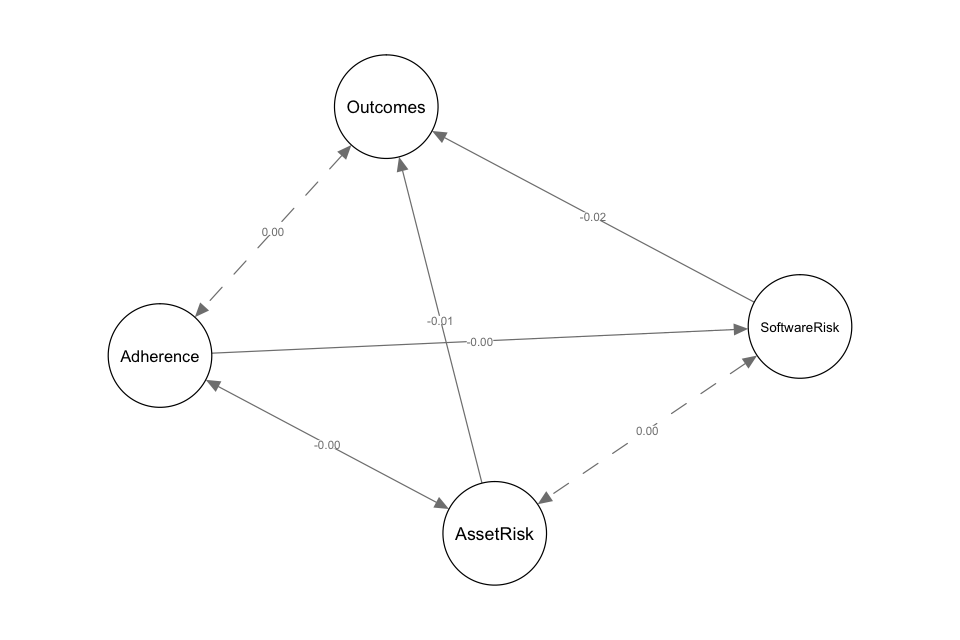
\includegraphics[width=\columnwidth]{modelzeroB.png}
 	\caption{Structural and Measurement Model Overview}
 	\label{fig:model_constructs}
 \end{figure}
  
\begin{table*}[!htbp] \centering 
	\caption{Lavaan Syntax} 
	\label{tab:model_lavaan_syntax} 
	\begin{small}
		\begin{tabular}{p{.75cm}p{1.25cm}p{1.5cm}p{3.5cm}p{2.5cm}} 
			&&&&\\[-1.8ex]\hline 
			\hline&&&& \\[-1.8ex] 
			Syntax & Symbol & Name & Description & Example \\ 
			\hline &&&&\\[-1.8ex]  
			$=\sim$	& $\bigcirc \rightarrow \Box$ & is measured by & $=\sim$ specifies how a latent variable (left side) is measured by the constituent variables listed on the right side & $SoftwareRisk =\sim SLOC + Churn$\\	
			 $\sim$ & $\bigcirc \leftarrow \bigcirc$ & regression & $\sim$ specifies a regression of the dependent variable on the left-hand side to the independent variables on the right hand side of the expression. & Outcomes $\sim$ SoftwareRisk $+$ AssetImpact  \\	
			 $\sim\sim$ & $\bigcirc \leftrightarrow \bigcirc$ $\Box \leftrightarrow \Box$ & undirected covariance & model a covariance relationship, but leave the direction of influence unspecified. When  & $AssetRisk \sim\sim Adherence$\\
			\hline &&&&\\[-1.8ex] 
			\hline &&&&\\[-1.8ex] 
		\end{tabular} 
	\end{small}
\end{table*} 


\begin{figure*}
	\centering
%	\begin{subfigure}{.5\textwidth}
		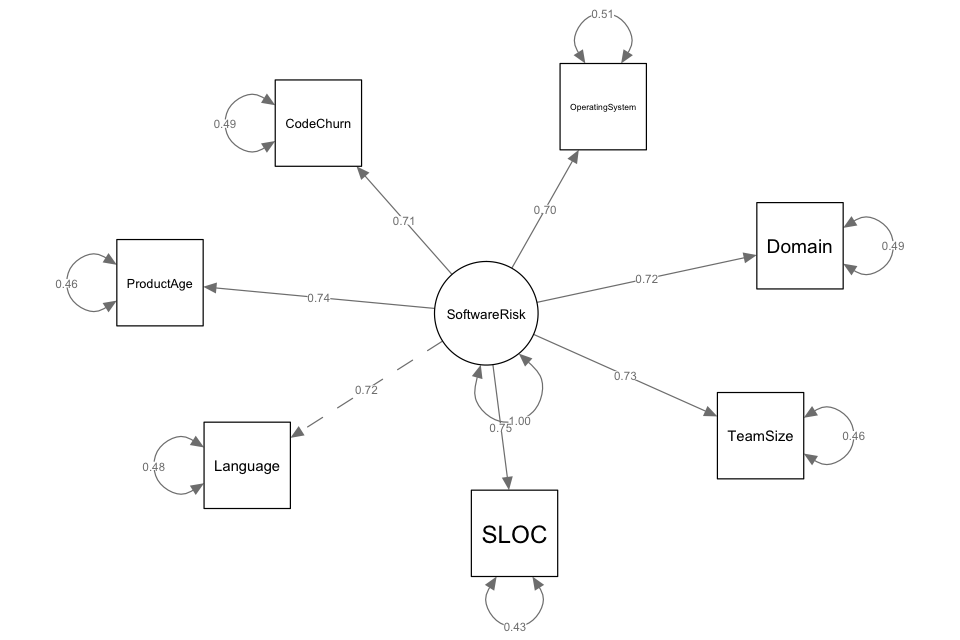
\includegraphics[width=1\textwidth]{syntax_swrisk_asmeasuredby.png}
		\caption{Graphical display of lavaan syntax for SoftwareRisk $=\sim$ Theorized measurement variables from Table  \ref{tab:model_spef_metrics}}
		\label{fig:model_example_syntax_asmeasuredby}	
%	\end{subfigure}%
%	\begin{subfigure}{.5\textwidth}		
%		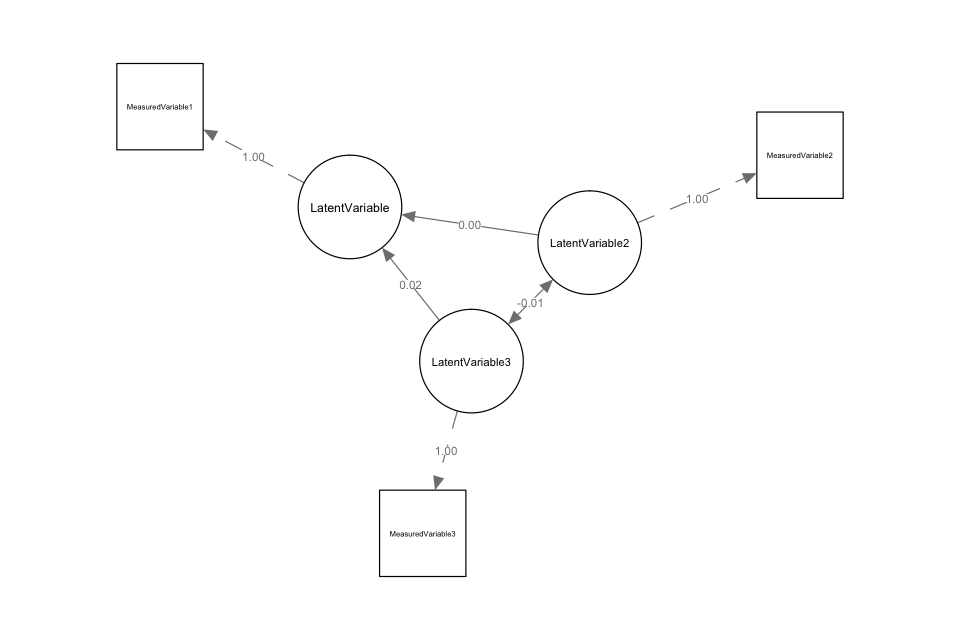
\includegraphics[width=.5\columnwidth]{syntax_latentregress.png}
%		\caption{Graphical display of lavaan syntax for $LatentVariable \sim LatentVariable2 + LatentVariable3$ (with measured variables)}
%		\label{fig:model_example_syntax_latentregress}	
%	\end{subfigure}		
\end{figure*}

%\begin{figure}
% \includegraphics[width=\columnwidth]{modelcaoscto}
%	\caption{Model Constructs and Sub-Constructs}
%	\label{fig:model_constructs_phases}
%\end{figure}
